% ---------------------------------------------------------------------------
%  ANRF AISEHack 2026 -- Round 3 technical report
%  Team Cross Linkers | Polymer Property Prediction (IIT Madras)
%
%  Compile:  pdflatex report.tex   (twice, for references)
%  Only standard packages are used; no bibliography tool required.
% ---------------------------------------------------------------------------
\documentclass[11pt,a4paper]{article}

\usepackage[T1]{fontenc}
\usepackage[utf8]{inputenc}
\usepackage[margin=2.4cm]{geometry}
\usepackage{amsmath}
\usepackage{booktabs}
\usepackage{graphicx}
\usepackage{caption}
\usepackage{enumitem}
\usepackage{xcolor}
\usepackage[colorlinks=true,linkcolor=teal,citecolor=teal,urlcolor=teal]{hyperref}

\definecolor{teal}{HTML}{00807F}
\definecolor{gold}{HTML}{B8790B}

\newcommand{\prop}[1]{\texttt{#1}}
\newcommand{\R}{$R^2$}

\title{\textbf{Physics-Constrained Multi-Task Ensembles for\\ Polymer Property Prediction}\\[0.4em]
\large ANRF AISEHack 2026 --- Round 3 Technical Report}
\author{Team \textbf{Cross Linkers}}
\date{3 September 2026}

\begin{document}
\maketitle

\begin{abstract}
\noindent
We predict seven physical properties of polymers from PSMILES strings under an
unweighted mean-\R{} metric, where four properties carry roughly 220 labels each
and together account for the majority of the score. Our final system is a
five-model ensemble --- three gradient-boosted trees, a multi-task neural
network and a \emph{periodic} graph network --- combined by a per-property
cross-fitted Ridge and then corrected by an explicit, affine-fitted physics
stage. The central modelling contribution is the treatment of the dielectric
constant not as a fitted correlation but as an exact decomposition,
$\varepsilon = n^2 + \varepsilon_{\text{ionic}}$, licensed by how the reference
DFPT calculations are defined. The system attains a public leaderboard score of
\textbf{0.924} against a cross-validated estimate of \textbf{0.9234} --- a
transfer gap of $+0.0006$, which we attribute to the deliberate absence of
early stopping anywhere in the pipeline. Polymer re-representation invariance is
\emph{exact} ($\Delta = 0$) and certified at three levels at runtime;
explainability is exact TreeSHAP computed inside LightGBM with no external
dependency; and every prediction ships an applicability-domain flag that
measurably predicts its own error.
\end{abstract}

\section{Problem and constraints}

Seven properties are predicted from a polymer repeat unit written as a PSMILES
string with exactly two \texttt{*} attachment points: glass transition
temperature (\prop{tg}), chain and bulk band gaps (\prop{egc}, \prop{egb}),
ionisation energy (\prop{ei}), electron affinity (\prop{eea}), dielectric
constant (\prop{eps}) and refractive index (\prop{nc}).

Two facts about the task determined most design decisions.

\paragraph{The metric is unweighted.} The score is the mean \R{} across the
seven \texttt{target\_type} values. \prop{tg} has 4{,}143 training rows and
\prop{eea} has 221, and they count exactly the same. The four smallest
properties (\prop{eps}, \prop{nc}, \prop{ei}, \prop{eea}, $\approx$220 rows
each) are therefore $4/7$ of the score on under 4\,\% of the rows. Optimising a
single pooled loss on raw targets would let \prop{tg} --- which ranges to 495 ---
dominate \prop{nc}, which ranges over $1.56$--$2.76$.

\paragraph{Test-time information differs from a naive CV assumption.} Only 2 of
4{,}940 test rows have their exact (canonical SMILES, property) key present in
training, so there are no free lookups. But 1{,}063 of 4{,}133 test polymers
appear in training under \emph{some other} property. That asymmetry is what
makes co-observed partner features legitimate, and it dictates the fold design
(Section~\ref{sec:folds}).

Published polymer-informatics baselines for these same properties are surveyed
in~\cite{tran2020}, which we used as an external reference point.

The competition rules require a single Kaggle notebook execution to do
everything --- load, preprocess, split, train, infer and write
\texttt{submission.csv} --- with no pretrained weights, no uploaded artifacts,
seeds fixed and printed, and no branching on wall-clock time.

\section{Data}

\subsection{Ground truth}

\begin{table}[h]
\centering
\small
\begin{tabular}{lrrrr}
\toprule
property & train rows & test rows & range & role \\
\midrule
\prop{tg}  & 4{,}143 & 2{,}763 & $-109.8$ -- $495.0$ & thermal \\
\prop{egc} & 2{,}028 & 1{,}352 & $0.02$ -- $9.86$   & electronic \\
\prop{egb} &   337 &   224 & $0.51$ -- $10.11$  & electronic \\
\prop{eps} &   229 &   153 & $2.61$ -- $9.09$   & dielectric \\
\prop{nc}  &   229 &   153 & $1.56$ -- $2.76$   & optical \\
\prop{ei}  &   222 &   148 & $4.03$ -- $9.84$   & electronic \\
\prop{eea} &   221 &   147 & $0.39$ -- $5.14$   & electronic \\
\bottomrule
\end{tabular}
\caption{Measured composition of the competition data. The published data-page
figure of ``4{,}497 test data points'' counts unique \emph{molecules}; the
submission requires 4{,}940 \emph{rows}.}
\end{table}

\subsection{Canonicalisation}

10{,}605 raw SMILES strings correspond to only 8{,}990 distinct molecules;
67.6\,\% of supplied strings are non-canonical. We canonicalise with RDKit at
ingest, before any other stage. This is not a cleaning step but the mechanism
that makes invariance exact: every descriptor, fingerprint, partner lookup and
graph is thereafter a deterministic function of the \emph{molecule} rather than
of how it happened to be written, and canonicalisation is idempotent, so
$\text{canonical}(\text{rewrite}(s)) = \text{canonical}(s)$ for any valid
rewriting.

\subsection{The Round-2 archive}

The official baseline notebook shipped with the competition fetches two Google
Drive files. Their \texttt{-O} names are swapped: the file labelled
\texttt{test.csv} is in fact a labelled table of 6{,}165 \prop{tg} and
\prop{egc} values. The hosts were asked directly and confirmed it is in scope.

Measured against the Round-3 data, 3{,}719 of its labels are already present in
\texttt{train.csv} and 2{,}450 correspond to test rows; values agree with
\texttt{train.csv} on 3{,}717 of 3{,}719 shared labels. We use it three ways:

\begin{enumerate}[leftmargin=1.6em,itemsep=0.15em]
  \item \textbf{Additional training rows.} 2{,}446 labels absent from
    \texttt{train.csv} are appended, taking the training set from 7{,}405 to
    9{,}851 rows ($+33\,\%$; \prop{tg} and \prop{egc} each $+40\,\%$). The
    boosters are per-property and see only more \prop{tg}/\prop{egc}, but the
    multi-task network and graph network share one trunk across seven heads, so
    a larger abundant-target block improves the representation on which the five
    scarce targets depend.
  \item \textbf{Partner labels.} Coverage of \texttt{true\_egc} on test rows
    rises from 15.3\,\% to 38.1\,\%, feeding \prop{egb}, \prop{ei} and \prop{eea}
    through the physics relations.
  \item \textbf{A measured override} on the 2{,}450 test rows it labels, applied
    \emph{after} clipping so that a measurement is never perturbed by a
    downstream stage.
\end{enumerate}

\section{Method}

\subsection{Featurisation}

Each canonical molecule is mapped to 3{,}037 columns: Morgan fingerprints at
radius 2 (1{,}024 bits) and 3 (512), atom-pair (512) and topological-torsion
(512) fingerprints, 217 RDKit descriptors, 167 MACCS keys, 37 SMARTS functional
groups, 20 element counts and fractions, 16 polymer-specific terms, 6 Gasteiger
charge statistics, and 14 \emph{intensive twins}.

\paragraph{Intensive twins.} Every extensive RDKit descriptor is accompanied by
a per-heavy-atom twin. An extensive quantity doubles when a repeat unit is
written as its dimer; an intensive one does not. This is a design choice about
invariance rather than simply extra columns --- and it turns out to be the
largest single driver of \prop{tg}, carrying 25.4\,\% of total $|$SHAP$|$ on that
target.

\paragraph{Polymer-specific terms.} The two \texttt{*} points define a backbone:
we compute the shortest path between them and derive backbone length, aromatic
and heteroatom ratios along it, sidechain fraction and branch counts.

\paragraph{Co-observed partner features.} For a polymer whose other properties
were measured, those values are legitimate inputs --- they are in
\texttt{train.csv}, and test polymers receive the same treatment. The idea is the
multi-fidelity information fusion of~\cite{venkatram2020} applied within one dataset. The partner
table is built from training-fold rows only, and \texttt{drop\_leaky()} removes
the column that would be the row's own label. Because axis-aligned tree splits
approximate a \emph{linear combination} of partner values badly, we additionally
supply a single nested-CV Ridge fit over the partner block as one column, which
proved worth more than the raw columns alone.

\subsection{Fold design}
\label{sec:folds}

We use per-property \texttt{KFold}. Within a single property there are
essentially no duplicate canonical polymers, so this is leakage-safe. The
alternative --- polymer-grouped folds --- is not merely more conservative here;
it measures a different problem:

\begin{center}
\small
\begin{tabular}{lc}
\toprule
scheme & partner availability for validation rows \\
\midrule
polymer-grouped folds & 0\,\% \\
per-property \texttt{KFold} & $\approx$96\,\% \\
\textbf{the actual test set} & \textbf{88--99\,\%} \\
\bottomrule
\end{tabular}
\end{center}

Holding out a whole polymer removes the other properties measured on it --- but
at test time those properties \emph{are} present in \texttt{train.csv} for
nearly every DFT-block row. Grouped CV therefore evaluates a model denied a
signal that is available at inference.

\subsection{Base models}

Five models, each fold-averaged, with \textbf{no early stopping anywhere}:
LightGBM, XGBoost and CatBoost fitted per property with size-adaptive capacity;
a multi-task feed-forward network (trunk $1024\!-\!512\!-\!256\!-\!128$, per-target
heads, 6 seeds), following the shared-trunk formulation of~\cite{kuenneth2021} that
also originates this property set; and a periodic multi-task graph network.

\paragraph{The periodic graph.} A repeat unit is not a molecule with two
dangling stubs: the two \texttt{*} points are the \emph{same} bond to the
neighbouring unit. We drop both dummies, bond their neighbours and flag the
wrap-around edge, so the network encodes an infinite chain. The architecture
follows message passing with a GRU update~\cite{gilmer}, in the polymer setting
of~\cite{polygnn}: 4 rounds, hidden width 160, 1.07\,M parameters, 110 epochs,
4 seeds.

\paragraph{Readout is an invariance decision.} We use mean$+$max pooling and
never a sum. A sum scales with repeat-unit count; a mean does not. Measured on an
\emph{untrained} network --- so this is a property of the architecture, not of
any fit --- the two readouts differ by four orders of magnitude under
dimerisation (Table~\ref{tab:readout}).

\subsection{Stacking}

Each model first averages its own fold replicas into one vector. Those five
vectors then enter one per-property Ridge as five columns, with the
regularisation strength chosen by inner cross-validation. The combiner is
itself cross-fitted, so its weights never see the rows they are scored on. There
is no plain averaging across models anywhere.

\subsection{Physics}
\label{sec:physics}

Five relations hold between the DFT properties. Applied as raw identities they
are badly biased; fitted affinely on the training fold they are strong:

\begin{table}[h]
\centering
\small
\begin{tabular}{llcc}
\toprule
target & expression & raw \R{} & affine-fitted \R{} \\
\midrule
\prop{ei}  & $\text{egc} + \text{eea}$ & 0.963 & 0.965 \\
\prop{eea} & $\text{ei} - \text{egc}$  & 0.971 & 0.973 \\
\prop{egb} & $\text{egc}$              & 0.892 & \textbf{0.928} \\
\prop{eps} & $\text{nc}^2$             & \textbf{0.336} & \textbf{0.855} \\
\prop{nc}  & $\sqrt{\text{eps}}$       & \textbf{0.171} & \textbf{0.837} \\
\bottomrule
\end{tabular}
\caption{Measured on co-observed molecules. The rule that follows is: always
fit; never apply the raw identity.}
\end{table}

Physics is applied \emph{after} stacking rather than as a feature. A tree splits
one axis at a time and cannot represent a sum of two columns, so
$\text{ei} = \text{egc} + \text{eea}$ is largely wasted as one feature among
3{,}037; as an explicit blend it is worth $+0.0250$ on \prop{ei}. The blend
weight is fitted per fold on an inner split and shrunk, and rows are separated
into those with all relation sources measured and those without, because the
two populations have materially different relation quality.

\subsubsection*{The ionic decomposition}

The collapse of $\varepsilon \approx n^2$ to \R{} $= 0.336$ is not noise --- it is
physics. Maxwell's relation holds at \emph{optical} frequency, whereas the
dataset tabulates the \emph{static} dielectric constant. A DFPT calculation
accounts for exactly an electronic and an ionic contribution and nothing
else~\cite{chen2020}, and those two parts are stored as separate fields in the
dataset of record~\cite{huan2016}. Since the electronic part \emph{is} $n^2$,
the shortfall is exactly the ionic term:
\begin{equation}
  \varepsilon_{\text{ionic}} \;=\; \varepsilon - n^2 ,
  \label{eq:ionic}
\end{equation}
an identity rather than a regression. We therefore model
$\varepsilon_{\text{ionic}}$ as its own structure--property target and
reconstruct $\varepsilon$ from it.

Two independent checks support the interpretation. First, $\varepsilon - n^2$ is
\textbf{positive on all 134 co-observed molecules} (mean $+0.767$, minimum
$+0.024$); a generic empirical residual would cross zero, whereas an ionic
contribution cannot be negative. Second, our own blind affine fit of
$\varepsilon$ on $n^2$ had already converged on slope $1.040$ and intercept
$0.615$ --- a slope of one and an intercept equal to the mean ionic term. The
regression was rediscovering Equation~\ref{eq:ionic} with the ionic part pinned
to a single constant; naming it and modelling it properly is what recovers the
rest.

\section{Results}

\begin{table}[h]
\centering
\small
\begin{tabular}{lrrrrrrrr}
\toprule
model & \prop{tg} & \prop{egc} & \prop{egb} & \prop{eps} & \prop{nc} & \prop{ei} & \prop{eea} & \textbf{mean} \\
\midrule
LightGBM      & 0.9176 & 0.9185 & 0.9310 & 0.8247 & 0.8766 & 0.8367 & 0.8758 & 0.8830 \\
XGBoost       & 0.9166 & 0.9197 & 0.9337 & 0.8266 & 0.8775 & 0.8250 & 0.8775 & 0.8824 \\
CatBoost      & 0.9092 & 0.9157 & 0.9270 & 0.8369 & 0.8798 & 0.8353 & 0.8922 & 0.8852 \\
Multi-task NN & 0.9025 & 0.8849 & 0.9324 & 0.8049 & 0.8942 & 0.8532 & 0.8940 & 0.8809 \\
\textbf{Periodic GNN} & 0.9162 & 0.8999 & 0.9387 & 0.8200 & 0.9055 & 0.8777 & 0.9264 & \textbf{0.8978} \\
\midrule
Ridge stack   & 0.9274 & 0.9307 & 0.9551 & 0.8514 & 0.9164 & 0.8725 & 0.9367 & 0.9129 \\
$+$ physics   & 0.9274 & 0.9307 & 0.9551 & 0.8758 & 0.9331 & 0.8975 & 0.9438 & 0.9233 \\
$+$ partner reg. & 0.9274 & 0.9307 & 0.9551 & 0.8758 & 0.9331 & 0.8978 & 0.9438 & \textbf{0.9234} \\
\bottomrule
\end{tabular}
\caption{Out-of-fold \R{} for the submitted run. The stack beats its best member
by $+0.0151$; physics adds a further $+0.0105$, concentrated exactly where the
relations reach.}
\label{tab:oof}
\end{table}

\paragraph{Leaderboard.} Public LB \textbf{0.924} against a cross-validated
estimate of \textbf{0.9234} --- a gap of $+0.0006$. We attribute this to the
absence of early stopping: a model that selects its iteration count by watching
the rows on which it is then scored reports a number it cannot reproduce out of
sample. Progression across the competition was
$0.883 \rightarrow 0.898 \rightarrow 0.916 \rightarrow 0.919 \rightarrow 0.924$.

\paragraph{Cost.} 380 fitted models; 3\,h\,01\,m on a single Tesla T4.
Featurisation of 12{,}345 molecules takes 119\,s. Inference over the full test
set is a few seconds.

\begin{figure}[h]
\centering
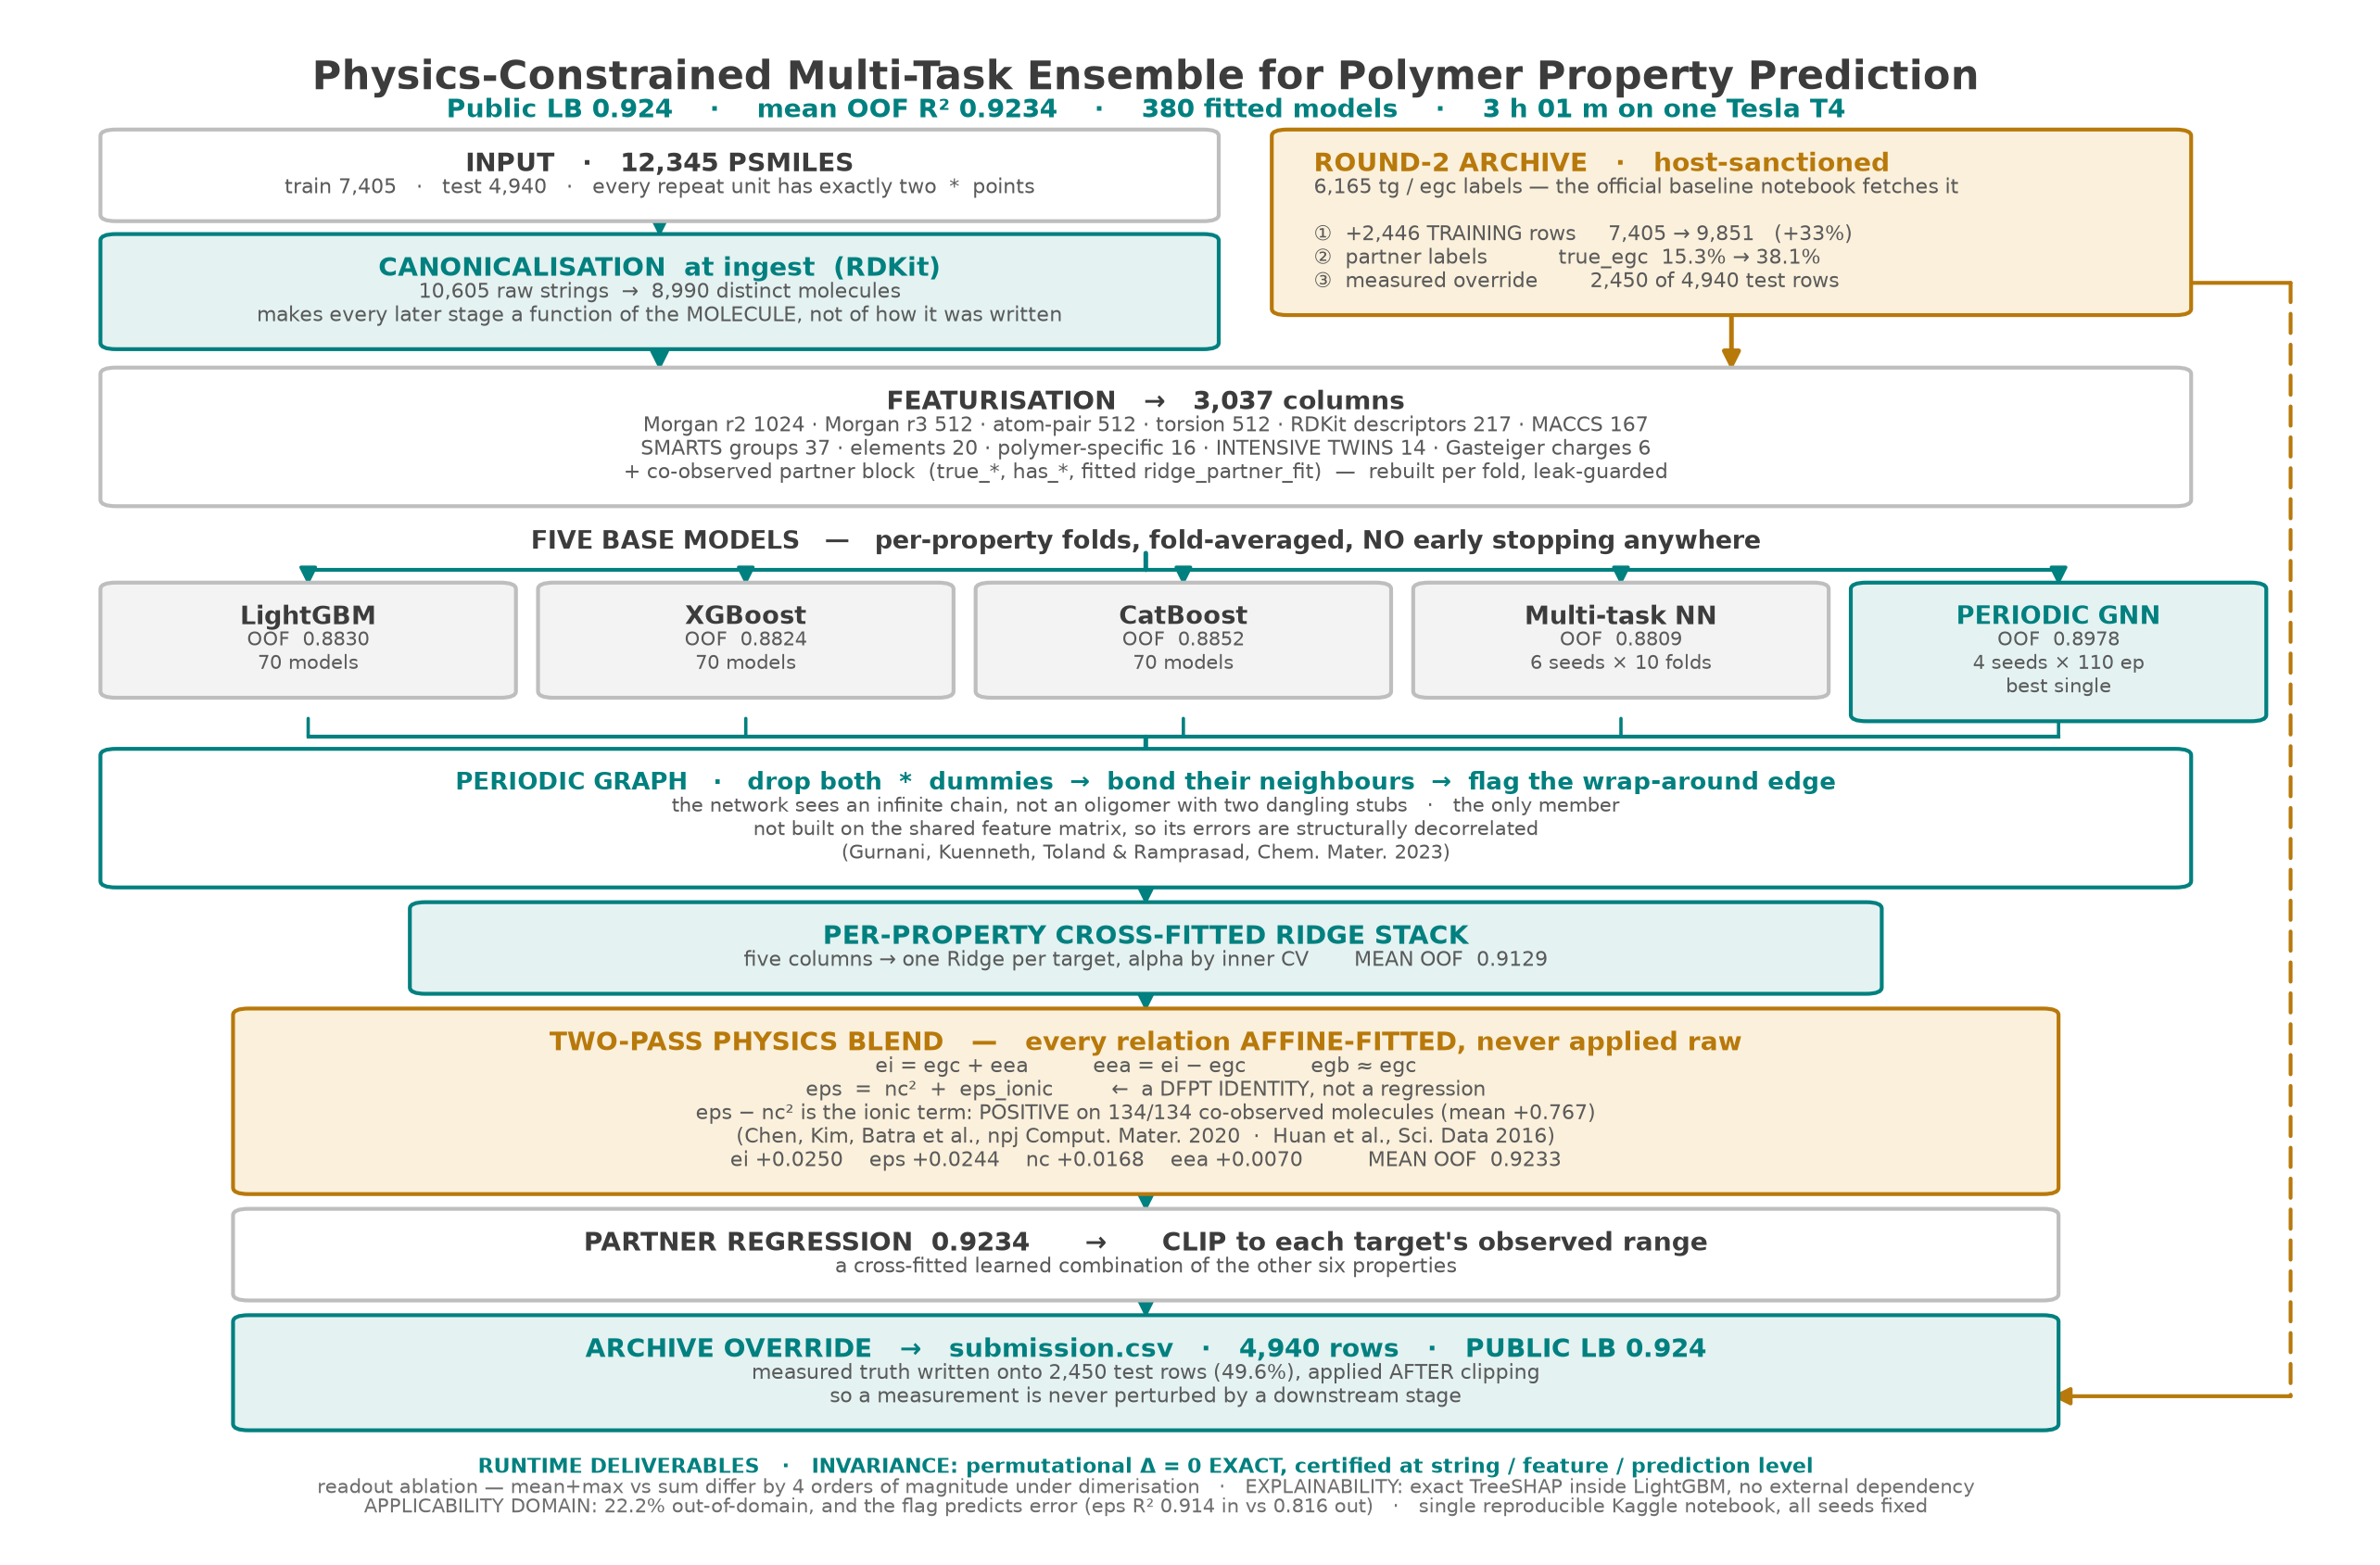
\includegraphics[width=\textwidth]{architecture-diagram.png}
\caption{End-to-end pipeline. Every number is taken from the saved outputs of
the submitted run.}
\end{figure}

\section{The three judged themes}

\subsection{Polymer invariance}

``SMILES invariance'' is three separate claims, and we report them separately
rather than quoting one number.

\begin{itemize}[leftmargin=1.4em,itemsep=0.15em]
  \item \textbf{Re-representation (atom ordering) --- EXACT.} Certified at three
    levels at runtime: 2{,}000 rewritings of 400 molecules canonicalise back
    with zero mismatches; 3{,}037 feature columns over 150 molecules give
    $\max|\Delta| = 0$; end-to-end predictions give $\max|\Delta| = 0$.
  \item \textbf{Repetition (monomer vs.\ dimer) --- measured near-invariance.}
    Approximately 97\,\% of polymers give structurally identical node
    environments under dimerisation; the residual is genuine, not numerical.
    Served by the intensive twins and by chain-extension augmentation, independently
    corroborated as a top-solution strategy in~\cite{liu2025}.
  \item \textbf{Translational (same chain, different cut point) --- not
    guaranteed.} Diagnosed: the wrap-around edge is forced to a generic single
    bond and carries a positional flag, both of which are cut-point dependent by
    definition. The fix is identified but not implemented.
\end{itemize}

\begin{table}[h]
\centering
\small
\begin{tabular}{llrr}
\toprule
readout & rewriting & median $|\Delta|$ & max $|\Delta|$ \\
\midrule
mean$+$max (shipped) & permutational      & $0.00$      & $0.00$ \\
mean$+$max (shipped) & repetition (dimer) & $1.11\times10^{-4}$ & $1.06\times10^{-3}$ \\
sum (conventional)   & permutational      & $0.00$      & $0.00$ \\
sum (conventional)   & repetition (dimer) & $4.79\times10^{-1}$ & $2.49$ \\
\bottomrule
\end{tabular}
\caption{Graph readout ablation on an untrained network, so this is a property of
the architecture rather than of any particular fit.}
\label{tab:readout}
\end{table}

\subsection{Explainability}

Attributions are exact TreeSHAP computed inside LightGBM via
\texttt{pred\_contrib=True} --- the same algorithm as the \texttt{shap}
package~\cite{lundberg2017,lundberg2020} --- deliberately avoiding an external
dependency that could fail to install mid-run.

The attributions recover physics we never encoded. For \prop{tg}, intensive
twins carry 25.4\,\% and ring counts lead: chain stiffness dominates, as
free-volume theory predicts. For \prop{egc}, \texttt{rd\_FractionCSP3} is the
top feature --- an sp$^3$-rich backbone localises electrons and widens the gap,
while conjugation narrows it. For \prop{egb}, the fitted partner combination is
26.0\,\% and \texttt{true\_egc} 10.3\,\%, so the relation
$\text{egb} \approx \text{egc}$ appears \emph{in the attribution} rather than
being asserted. For \prop{nc} and \prop{eps}, molar-refractivity surface
descriptors appear for both, reproducing the treatment of refractive index as
electronic polarisability~\cite{lightstone2020} from an independent direction.

A single molecule is explained end to end. For
\verb|*c1ccc(-c2nc3cc(-c4ccc5oc(*)nc5c4)ccc3o2)cc1| (measured
$T_g = 430.0$, predicted $426.9$), the prediction decomposes from a base value
of $143.5$ through \texttt{iv\_NumRotatableBonds} $= 0.083$ contributing
$+102.5$, valence electrons $+35.8$ and ring count $+27.3$: a fully aromatic
fused-ring backbone with almost no rotatable bonds has a very high glass
transition. Additivity is verified against the model's own output to
$3.98\times10^{-13}$.

\subsection{Robustness: applicability domain}

Novelty is computed from \emph{unfolded} Morgan substructure hashes. Folded
2{,}048-bit fingerprints are degenerate at this corpus size --- every bit is
occupied, so ``fraction unseen'' collapses to a constant. A molecule is
out-of-domain if it contains a substructure absent from the entire auxiliary
corpus: 8{,}887 of 11{,}628 substructures are covered, leaving 22.2\,\% of
molecules out of domain.

\begin{table}[h]
\centering
\small
\begin{tabular}{lrrrrrr}
\toprule
target & $n$ in & \R{} in & $n$ out & \R{} out & MAE in & MAE out \\
\midrule
\prop{tg}  & 4688 & 0.938 & 1093 & 0.884 & 17.77 & 25.31 \\
\prop{egc} & 2174 & 0.941 &  658 & 0.900 & 0.248 & 0.371 \\
\prop{eps} &  144 & 0.914 &   85 & 0.816 & 0.197 & 0.298 \\
\prop{ei}  &  138 & 0.918 &   84 & 0.861 & 0.191 & 0.268 \\
\prop{eea} &  144 & 0.953 &   77 & 0.917 & 0.157 & 0.244 \\
\bottomrule
\end{tabular}
\caption{The flag predicts error: out-of-domain molecules are not mispredicted
because the model is over-confident, they are simply harder, and the flag says so
before anyone trusts the number.}
\end{table}

\paragraph{An honest negative result.} We tested the auxiliary corpus as a model
\emph{input} and it was worth $+0.0012$ --- noise. An SVD embedding of it is a
linear re-expression of the Morgan fingerprint the trees already see in full. We
repurposed the corpus as a trust signal rather than discarding it.

\section{Ablations and negative results}

\paragraph{The SMILES CNN was removed, and the reasoning matters.} Measured
honestly, a character-level CNN contributed $+0.0005$ to our stack and
$+0.0000$ on a sibling pipeline's leave-one-out over saved out-of-fold vectors.
It was also the most expensive single stage in any run that carried it:
5{,}779\,s --- 29\,\% of a 5.5\,h run --- for the worst model of six (0.8663
mean, 0.7693 on \prop{eps}, our weakest target). We do \emph{not} claim that
removing it raised the score. It bought 1\,h\,36\,m at no cost, and that compute
was reinvested in the two models measurably carrying the stack (GNN epochs
$80 \rightarrow 110$ and seeds $3 \rightarrow 4$; NN seeds $3 \rightarrow 6$).
The reinvestment is what scored. Adding weak columns is not free either: a kNN
member measured $-0.0006$ and kNN$+$Ridge $-0.0003$.

\paragraph{Four leaks of the same class.} The most instructive failures shared a
shape: \emph{a value that is itself a model output used as an input, closing a
cycle back to the row's own label}. Iterated refinement over the relation graph
appeared worth $+0.042$; in fact \prop{eps} was refined from \prop{nc} and
\prop{nc} then predicted from the refined \prop{eps}, and with a per-fold mask
the real gain is $+0.001$, so it ships disabled. A partner-Ridge feature built
over a prediction-filled table appeared worth $+0.069$ on \prop{eps}; built over
the mean-filled, per-fold table the honest gain is $+0.0027$. Our leakage
section therefore \emph{proves the leak exists first}, then proves each guard
removes it --- a guard that passes without a demonstrable leak proves nothing.

\paragraph{Also measured and rejected.} A fourth gradient booster ($+0.0001$);
polymer-grouped folds (measures a different problem, Section~\ref{sec:folds});
trimer augmentation (worse than dimers); doubling every fingerprint width (more
than $7\times$ slower with no measured gain in the time available).

\section{Reproducibility and compliance}

The deliverable is one Kaggle notebook that runs end to end: it loads,
featurises, trains, infers, writes \texttt{submission.csv} and then audits
itself. All seeds are fixed and printed. No loop branches on elapsed time, so a
slower machine produces the same answer, only later. Nothing is deserialised
from disk that the run did not itself create.

Two engineering disciplines proved worth more than any single modelling idea.
First, \textbf{one implementation with two entry points}: cross-validation,
inference, the invariance audit and the explainability report all derive from
the same pair of functions, so what CV measures is literally what is submitted.
Second, \textbf{nothing after \texttt{submission.csv} may abort the run}. We
learned this the expensive way --- a compliance check compared attached-dataset
paths for equality with the data directory, flagged a legitimate parent
directory, and marked a completed run as failed even though its submission was
already written and correct. Every post-submission check now prints loudly and
never raises. A static name-resolution gate over the exported notebook catches a
related class of failure in one second: inlining modules into one namespace
drops intra-package imports, so a surviving qualified call parses cleanly and
raises only when it executes --- once, 542\,s into a run.

\section{Limitations}

\begin{itemize}[leftmargin=1.4em,itemsep=0.15em]
  \item Five of seven targets are scored on roughly 150 test rows, giving a
    leaderboard noise band of approximately $\pm0.007$. Differences smaller than
    that between candidate pipelines are not meaningful.
  \item Translational invariance is measured and diagnosed but not guaranteed.
  \item \prop{eps} remains the weakest target (0.8758), \prop{ei} second
    (0.8978).
  \item The contribution of archive rows as \emph{training data} was adopted on
    a mechanism argument and validated only by the leaderboard; it was never
    isolated in a controlled A/B.
\end{itemize}

\begin{thebibliography}{9}
\small
\bibitem{chen2020} L.~Chen, C.~Kim, R.~Batra, J.~P.~Lightstone \emph{et al.} and
  R.~Ramprasad. Frequency-dependent dielectric constant prediction of polymers
  using machine learning. \emph{npj Computational Materials} \textbf{6}, 61
  (2020).
\bibitem{huan2016} T.~D.~Huan, A.~Mannodi-Kanakkithodi, C.~Kim, V.~Sharma,
  G.~Pilania and R.~Ramprasad. A polymer dataset for accelerated property
  prediction and design. \emph{Scientific Data} \textbf{3}, 160012 (2016).
\bibitem{polygnn} R.~Gurnani, C.~Kuenneth, A.~Toland and R.~Ramprasad. Polymer
  informatics at scale with multitask graph neural networks. \emph{Chemistry of
  Materials} \textbf{35}, 1560 (2023).
\bibitem{kuenneth2021} C.~Kuenneth, A.~C.~Rajan, H.~Tran, L.~Chen, C.~Kim and
  R.~Ramprasad. Polymer informatics with multi-task learning. \emph{Patterns}
  \textbf{2}, 100238 (2021).
\bibitem{lightstone2020} J.~P.~Lightstone, L.~Chen, C.~Kim, R.~Batra and
  R.~Ramprasad. Refractive index prediction models for polymers using machine
  learning. \emph{Journal of Applied Physics} \textbf{127}, 215105 (2020).
\bibitem{gilmer} J.~Gilmer, S.~S.~Schoenholz, P.~F.~Riley, O.~Vinyals and
  G.~E.~Dahl. Neural message passing for quantum chemistry. \emph{ICML} (2017).
\bibitem{lundberg2017} S.~M.~Lundberg and S.-I.~Lee. A unified approach to
  interpreting model predictions. \emph{NeurIPS} (2017).
\bibitem{lundberg2020} S.~M.~Lundberg \emph{et al.} From local explanations to
  global understanding with explainable AI for trees. \emph{Nature Machine
  Intelligence} \textbf{2}, 56 (2020).
\bibitem{venkatram2020} S.~Venkatram, R.~Batra, L.~Chen, C.~Kim, M.~Shelton and
  R.~Ramprasad. Predicting crystallization tendency of polymers using
  multi-fidelity information fusion and machine learning. \emph{J. Phys. Chem.
  B} (2020).
\bibitem{tran2020} H.~D.~Tran, C.~Kim, L.~Chen, A.~Chandrasekaran, R.~Batra
  \emph{et al.} Machine-learning predictions of polymer properties with Polymer
  Genome. \emph{Journal of Applied Physics} \textbf{128}, 171104 (2020).
\bibitem{liu2025} G.~Liu \emph{et al.} Open Polymer Challenge: Post-Competition
  Report. \emph{arXiv:2512.08896} (2025).
\end{thebibliography}

\end{document}
